%====================================================
%	CHAPTER 5 - Allocation
%====================================================
\chapter{Controller Allocation}
\label{ch:allocation}
%====================================================
\section{Allocator slack}
\label{sec:allocation.slack}
%====================================================
Following the higher level control laws, a distribution algorithm is needed to \emph{allocate} out the desired virtual control inputs, $\vec{\nu}_d=[\mu\vec{F}~\mu\vec{\tau}]^T$, to commanded actuator positions, $u_c\in\mathbb{U}$. The allocation block, $B^\dagger(\mathbf{x},~\vec{\nu}_d,~t)$, from the control loop, Fig:\ref{fig:control-loop}, constructs physical actuator positions from the virtual control input. For regular, unconstrained control allocation the solution is posed as an optimization\footnote{\emph{Control Allocation by Johansen, et al. [2012]\cite{allocation}} \textbf{and} \emph{Control allocation for over actuated systems by Oppenheimer, et al. [2006]\cite{controlallocation}} both detail the nature of generalized nonlinear allocation loops.} problem; aiming to minimize deviation between the virtual and commanded control inputs, $\vec{\nu}_d$ \& $\vec{\nu}_c$ respectively.
\begin{equation}\label{eq:allocation-slack}
\underset{u\in\mathbb{U}^{12},~s\in\mathbb{R}^{6}}{min}\big(\norm{Q_s}\big)~~\text{such that}~~\vec{\nu}_d-\vec{\nu}_c=h(\mathbf{x}_e,t)-B(\mathbf{x},t,u)=s
\end{equation}
Where $Q_s$ is some cost function to prioritize the slack variable, $s$, requirements. Typically that cost function will just be the $L_2$ norm of the slack. In Eq:\ref{eq:allocation-slack} a generalized controller, $h(\mathbf{x}_e,t)$, is used; in the context of a 6-DOF control loop. That controller would combined virtual control inputs $\mu\vec{F}$ and $\mu\vec{\tau}$ for position and attitude control respectively. In the over-actuated case, there exists an entire family of suitable actuator positions $u$ which are all solutions to Eq:\ref{eq:allocation-slack}. The over-allocation solution is to introduce a secondary cost function\footnote{Or control objective.}, $J(\mathbf{x},t,u)$, into the optimization problem of Eq:\ref{eq:allocation-slack}.
\begin{equation}\label{eq:allocation-problem}
\underset{u\in\mathbb{U}^{12},~s\in\mathbb{R}^{6}}{min}\big(||Q_s||+J(\mathbf{x},u,t)\big)~~\text{such that}~~h(\mathbf{x}_e,t)-B(\mathbf{x},u,t)=s
\end{equation}
That secondary control objective $J(\mathbf{x},t,u)$ and its associated \emph{explicit} solution to Eq:\ref{eq:allocation-problem} is the subject of control allocation research. Not much work has been done on over-allocation for aerospace vehicles outside the field of satellite attitude control (Section:\ref{subsubsec:intro.lit.control.allocation} for examples). Often satellites are over actuated for the sake of fault tolerance and redundancy\cite{FTCallocation,discreteFTC}. Actuator rate constraints can be further introduced such that $u$ is limited by $\Delta u$, constraining sequential actuator position changes.
\begin{multline}
\therefore\underset{u\in\mathbb{U}^{12},~s\in\mathbb{R}^6}{min}\big(||Q_s||+J(\mathbf{x},u,t)\big)~~\text{s.t}~~h(\mathbf{x}_e,t)-B(\mathbf{x},u,t)=s\\\text{subject to}~~u=u_{n-1}+\Delta u,~\Delta u\in\mathbb{C}
\end{multline}
\par
Most control allocation paradigms assume a linear, multiplicative relationship with the effectiveness function, hence the abstraction layer which was introduced previously in Eq:\ref{eq:4.7}. The allocator effectiveness function, when abstracted to a linear matrix multiplication, reduces to:
\begin{equation}
\vec{\nu}_d=h(\mathbf{x}_e,t)\Longleftrightarrow B(\mathbf{x},u,t)=B(\mathbf{x},t)u=\vec{\nu}_c
\end{equation}
With $\vec{\nu}_d\text{~\&~}\vec{\nu}_c\in\mathbb{R}^n,~u\in\mathbb{U}\in\mathbb{R}^m,~B\in\mathbb{R}^{m\times n}$. That assumption makes addressing the allocation conceptually simpler, accommodating the use of inversion based allocation laws (Sec:\ref{subsec:control.allocation.inverse},\ref{subsec:control.allocation.weightedinverse},\ref{subsec:control.allocation.norminverse}). That abstraction to a multiplicative relationship with decomposed thrust components was suggested in Eq:\ref{eq:4.7}. The subsequent rotation "inversion" function, $R^\dagger(\mathbf{x},\vec{F}_i,t)$, to solve for physical actuator positions $(\Omega_i,\lambda_i,\alpha_i)$, is however as yet undefined.
\par
Assuming for the moment there is some allocation rule that, from $\vec{\nu}_d$, designs well four decomposed stabilizing 3-dimensional thrust vectors $\vec{T}_{1\rightarrow 4}$ to be produced by each motor module. It then follows that each of those four thrust vectors then relate\footnote{Using the quaternion analogue of rotation $\mathcal{F}^{M_i}\rightarrow\mathcal{F}^b$ from Eq:\ref{eq:motor-module-rotation.a}.} to their individual associated actuator positions through a quaternion \emph{rotation}:
\begin{subequations}
\begin{equation}\label{eq:4.101}
\vec{T}_i= Q_{M_i}\otimes\vec{T}(\Omega_i)\otimes Q_{M_i}^*~~~~\in\mathcal{F}^b
\end{equation}
\vspace{-16pt}
\begin{equation}\label{eq:4.101.b}
=Q_{z}(\sigma_i)Q_{y}(\alpha_i)Q_{x}(\lambda_i)\otimes \vec{T}(\Omega_i) \otimes Q_{x}^*(\lambda_i)Q_{y}^*(\alpha_i)Q_z^*(\sigma_i)
\end{equation}
Where each motor thrust vector, $\vec{T}(\Omega_i)$, is:
\begin{equation}
\vec{T}(\Omega_i)=\begin{bmatrix}
0\\
0\\
T(\Omega_i)
\end{bmatrix}=\begin{bmatrix}
0\\
0\\
C_T(J)\rho \Omega_i^2 D^4
\end{bmatrix}~~~~\in\mathcal{F}^{M_i}
\end{equation}
\end{subequations}
In the transformation Eq:\ref{eq:4.101} the angle $\sigma_i$ is an orthogonal $\hat{Z}$ transformation from $\mathcal{F}^b\rightarrow\mathcal{F}^{M_i''}$ from Eq:\ref{eq:motor-module-rotation.a}. The thrust function $T(\Omega_i)$ is the BEM theory equation using thrust coefficients, Eq:\ref{eq:aerodynamic-thrust}, in the direction of the rotor shaft's axis of rotation, bound to $\hat{Z}_{M_i}$. Seeing that quaternion rotation (\emph{transformation}) operators change the reference frame whilst retaining the vector operand's magnitude, it follows that $T(\Omega_i)$, and by extension the propeller speed $\Omega_i$, can be solved for:
\begin{subequations}
\begin{equation}
|\vec{T}_i|=\sqrt{\norm{[T_x~T_y~T_z]}}=\sqrt{T_x^2+T_y^2+T_z^2}=|T(\Omega_i)|=|C_T(J)\rho\Omega_i^2D^4|
\end{equation}
\vspace{-14pt}
\begin{equation}
\rightarrow \Omega_i=\sqrt{\frac{|\vec{T}_i|}{C_T(J)\rho D^4}}=\sqrt{\frac{\sqrt{T_x^2+T_y^2+T_z^2}}{C_T(J)\rho D^4}}
\end{equation}
\end{subequations}
Then reversing (or \emph{undoing}) the transformation from motor module to body frame in Eq:\ref{eq:4.101}:
\begin{subequations}
\begin{equation}
\vec{T}(\Omega_i)=Q_{z}^*(\sigma_i)Q_{y}^*(\alpha_i)Q_{x}^*(\lambda_i)\otimes \vec{T}_i \otimes Q_{x}(\lambda_i)Q_{y}(\alpha_i)Q_z(\sigma_i)~~~~\in\mathcal{F}^{M_i}
\end{equation}
\vspace{-14pt}
\begin{equation}
\rightarrow \vec{T}(\Omega_i)=Q_{M_i}^*\otimes \vec{T}_i \otimes Q_{M_i}~~~~\in\mathcal{F}^{M_i}
\end{equation}
\end{subequations}
Knowing only $\vec{T}(\Omega_i)$ and $\vec{T}_i$ in the motor frame and body frame respectively requires solving for a quaternion which relates the two. If both vectors are of unit length, $\hat{T}_i$ \& $\hat{T}(\Omega_i)$; then the following relationship can be exploited to find a relative quaternion:
\begin{subequations}
\begin{equation}
\hat{T}_i=\frac{\vec{T}_i}{|\vec{T}_i|}=\frac{\vec{T}_i}{\sqrt{T_x^2+T_y^2+T_z^2}}~~~~\in\mathcal{F}^b
\end{equation}
\vspace{-8pt}
\begin{equation}
\hat{T}(\Omega_i)=\frac{\vec{T}(\Omega_i)}{|\vec{T}(\Omega_i)|}=\frac{\vec{T}(\Omega_i)}{|C_T(J)\rho\Omega^2 D^4|}=\begin{bmatrix}
0 & 0 & 1
\end{bmatrix}^T~~~~\in\mathcal{F}^{M_i}
\end{equation}
\vspace{-4pt}
\begin{equation}\label{eq:vector-quaternion}
Q_{M_i}=\begin{bmatrix}
q_0\\
\vec{q}
\end{bmatrix}
=
\begin{bmatrix}
1+\hat{T}_i\cdot \hat{T}(\Omega_i)\\
-\hat{T}_i\times\hat{T}(\Omega_i)
\end{bmatrix}
\end{equation}
\end{subequations}
Where Eq:\ref{eq:vector-quaternion} is an extension of the inherent quaternion definition which rotates a vector around a single Euler axis, Eq:\ref{eq:quaternion-product}, when applied to two unit vectors. That quaternion can indeed be used to solve for relative pitch, roll and yaw Euler angles (Appendix:\ref{app:equations.quaternions}). The problem is that Eq:\ref{eq:vector-quaternion} solves for the \textbf{most direct, shortest path} rotation from one vector to another. In most cases, a sequenced Z-Y-X rotation is by no means the shortest possible path. As a result solutions for $[\phi,\theta,\psi]^T$ from Eq:\ref{eq:vector-quaternion} won't be meaningful for trying to resolve suitable servo positions $\lambda_i$ and $\alpha_i$.
\par
The associated $[\phi,~\theta,~\psi]^T$ solutions to Eq:\ref{eq:app-quaternion-eule} are then of no consequence in trying to solve for sequence of rotation angles\footnote{$\sigma_i$ is already known to be an orthogonal multiplicate\ldots} $[\lambda_i,~\alpha_i,~\sigma_i]^T$. Furthermore, when considering a sequenced Z-Y-X quaternion, no further insight can be extracted without applying cumbersome trigonometric inversions;
\begin{subequations}
\begin{equation}
Q_b=\begin{bmatrix}
cos\frac{\psi}{2}\\
0\\
0\\
sin\frac{\psi}{2}
\end{bmatrix}
\otimes
\begin{bmatrix}
cos\frac{\theta}{2}\\
0\\
sin\frac{\theta}{2}\\
0
\end{bmatrix}
\otimes
\begin{bmatrix}
cos\frac{\phi}{2}\\
sin\frac{\phi}{2}\\
0\\
0
\end{bmatrix}
\end{equation}
\begin{equation}
=
\begin{bmatrix}
c\frac{\psi}{2}c\frac{\theta}{2}c\frac{\phi}{2}+s\frac{\psi}{2}s\frac{\theta}{2}s\frac{\phi}{2}\\
c\frac{\psi}{2}c\frac{\theta}{2}s\frac{\phi}{2}-s\frac{\psi}{2}s\frac{\theta}{2}c\frac{\phi}{2}\\
c\frac{\psi}{2}s\frac{\theta}{2}c\frac{\phi}{2}+s\frac{\psi}{2}c\frac{\theta}{2}s\frac{\phi}{2}\\
s\frac{\psi}{2}c\frac{\theta}{2}c\frac{\phi}{2}-c\frac{\psi}{2}s\frac{\theta}{2}s\frac{\phi}{2}
\end{bmatrix}
=
\begin{bmatrix}
q_0\\
q_x\\
q_y\\
q_z
\end{bmatrix}
=
\begin{bmatrix}
q_0\\
\vec{q}
\end{bmatrix}
\end{equation}
\begin{equation}
\rightarrow\vec{T}_i=
\begin{bmatrix}
c\frac{\psi}{2}c\frac{\theta}{2}c\frac{\phi}{2}+s\frac{\psi}{2}s\frac{\theta}{2}s\frac{\phi}{2}\\
c\frac{\psi}{2}c\frac{\theta}{2}s\frac{\phi}{2}-s\frac{\psi}{2}s\frac{\theta}{2}c\frac{\phi}{2}\\
c\frac{\psi}{2}s\frac{\theta}{2}c\frac{\phi}{2}+s\frac{\psi}{2}c\frac{\theta}{2}s\frac{\phi}{2}\\
s\frac{\psi}{2}c\frac{\theta}{2}c\frac{\phi}{2}-c\frac{\psi}{2}s\frac{\theta}{2}s\frac{\phi}{2}
\end{bmatrix}
\otimes
\vec{T}(\Omega_i)
\otimes
\begin{bmatrix}
s\frac{\psi}{2}s\frac{\theta}{2}s\frac{\phi}{2}+c\frac{\psi}{2}c\frac{\theta}{2}c\frac{\phi}{2}\\
s\frac{\psi}{2}s\frac{\theta}{2}c\frac{\phi}{2}-c\frac{\psi}{2}c\frac{\theta}{2}s\frac{\phi}{2}\\
-c\frac{\psi}{2}s\frac{\theta}{2}c\frac{\phi}{2}-s\frac{\psi}{2}c\frac{\theta}{2}s\frac{\phi}{2}\\
c\frac{\psi}{2}s\frac{\theta}{2}s\frac{\phi}{2}-s\frac{\psi}{2}c\frac{\theta}{2}c\frac{\phi}{2}
\end{bmatrix}
\end{equation}
\end{subequations}
Instead; returning to rotation matrices for the inverse transformation and reiterating that Euler angle equivalents for the servos are; $[\phi,~\theta,~\psi]^T\iff [\lambda_i,~\alpha_i,~\sigma_i]^T$. It then follows (where \emph{$i^{th}$ motor subscripts} $1\rightarrow 4$ are implied):
\begin{subequations}
\begin{equation}
\vec{T}_i=\begin{bmatrix}
c\sigma & -s\sigma & 0\\
s\sigma & c\sigma & 0\\
0 & 0 & 1 
\end{bmatrix}
\begin{bmatrix}
c\alpha & 0 & s\alpha\\
0 & 1 & 0\\
-s\alpha & 0 & c\alpha
\end{bmatrix}
\begin{bmatrix}
1 & 0 & 0\\
0 & c\lambda & -s\lambda\\
0 & s\lambda & c\lambda
\end{bmatrix}\vec{T}(\Omega_i)
\end{equation}
\begin{equation}
\Rightarrow\vec{T}_i=\begin{bmatrix}
c\sigma c\alpha & c\sigma s\alpha s\lambda - s\sigma c\lambda & c\sigma s\alpha c\lambda + s\sigma s\lambda\\
s\sigma c\alpha & s\sigma s\alpha s\lambda + c\sigma c\lambda & s\sigma s\alpha c\lambda - c\sigma s\lambda\\
-s\alpha & c\alpha s\lambda & c\alpha c\lambda
\end{bmatrix}
\begin{bmatrix}
0\\
0\\
T(\Omega_i)
\end{bmatrix}
\end{equation}
\begin{equation}\label{eq:rotation-inverse}
\Rightarrow
\begin{bmatrix}
T_x\\
T_y\\
T_z
\end{bmatrix}
=\begin{bmatrix}
s\sigma s\lambda + c\sigma s\alpha c\lambda\\
s\sigma s\alpha c\lambda - c\sigma s\alpha\\
c\alpha c\lambda
\end{bmatrix}
T(\Omega_i)
\end{equation}
\end{subequations}
Where $\sigma$ is an orthogonal multiple which rotates the vector about the $\hat{Z}_b$ axis. The fact that the principle thrust vector $\vec{T}(\Omega_i)$ has only a $\hat{Z}_{M_i}$ component in the motor frame makes the solution for servo angles dramatically less complex to solve. Then Eq:\ref{eq:rotation-inverse} simplifies even further to the following four trigonometric relations respectively for each motor module:
\begin{equation}
\begin{bmatrix}
T_x\\
T_y\\
T_z
\end{bmatrix}
=
\begin{bmatrix}
\begin{bmatrix}
s\alpha c\lambda\\
-s\lambda \\
c\alpha c\lambda
\end{bmatrix}
,
\begin{bmatrix}
s\lambda\\
s\alpha c\lambda\\
c\alpha c\lambda
\end{bmatrix}
,
\begin{bmatrix}
-s\alpha c\lambda\\
s\lambda\\
c\alpha c\lambda
\end{bmatrix}
,
\begin{bmatrix}
-s\lambda\\
-s\alpha c\lambda\\
c\alpha c\lambda
\end{bmatrix}
\end{bmatrix}T(\Omega_i)~~~\text{for}~~i\in[1,~2,~3,~4]
\end{equation}
It then becomes a simple case of inverse trigonometry to solve for both $\lambda_i$ and $\alpha_i$ respectively, for the example case of $i=1$, the following holds true and can be similarly applied to the remaining motor modules.
\par
Using $T(\Omega_i)=||\vec{T}_i||$ and the four quadrant secondary arctangent2 function\footnote{More on the $arctan2$ function in Appendix:\ref{app:equations.quaternions}.}, $arctan2(x,y)$, for both inversion solutions to get full quadrature\footnote{Exploiting the fact that $arctan(x)=arcsin(x/\sqrt{1-x^2})$.} results:
\begin{subequations}
\begin{equation}
\lambda =  arctan2\bigg(-T_y,~\sqrt{||\vec{T}_i||^2-T_y^2}\hspace{2pt}\bigg)
\end{equation}
\vspace{-10pt}
\begin{equation}
\alpha_i = arctan2\big(T_x,~T_z\hspace{2pt}\big)
\end{equation}
\end{subequations}
Therefore, the secondary component of the control allocation block, $R^\dagger(\mathbf{x},\vec{T}_i,t)$ from Fig:\ref{fig:control-block} is then summarized as a single rotation inversion function (for motor module $i=1$):
\begin{equation}\label{eq:allocator-inersion}
\begin{bmatrix}
\Omega_i\\
\lambda_i\\
\alpha_i
\end{bmatrix}
=
R^\dagger(\mathbf{x},\vec{T}_i,t)=
\begin{bmatrix}
\Big(\sqrt{T_x\text{}^2+T_y\text{}^2+T_z\text{}^2}/C_T(J)\rho D^4\Big)\text{}^{\frac{1}{2}}\\
atan2(T_x\text{}^2,~||\vec{T}_i||\sqrt{||\vec{T}_i||\text{}^2-T_x\text{}^2})\\
-atan2(T_x,~T_z||\vec{T}_i||)
\end{bmatrix}
\end{equation}
Further simplifications could be drawn from the definitions of each element included in Eq:\ref{eq:allocator-inersion}, but it would just be superfluous as each servo angle can be solved for. At this stage the only remaining undefined component of the entire control block is the abstracted allocation algorithms, $B^\dagger(\mathbf{x},\vec{\nu}_d,t)$, which are now addressed\ldots
%====================================================
\subsection{Pseudo Inverse Allocator}
\label{subsec:control.allocation.inverse}
%====================================================
Conceptually the simplest control allocation solutions to Eq:\ref{eq:allocation-problem} stems from what are categorized as "inversion" based cost optimizations (the first three proposed allocators in Sec:\ref{subsec:control.allocation.inverse},\ref{subsec:control.allocation.weightedinverse} \& \ref{subsec:control.allocation.norminverse}). As alluded to previously, the requirements for inversion based allocation is that the effectiveness function $B(\mathbf{x},u,t)$ is a linear relationship which can be abstracted to $B(\mathbf{x},t)u$. The objective of inversion is that for the control problem $\vec{\nu}_c=B(\mathbf{x},t)u$ to find some matrix $B^\dagger(\mathbf{x},t)$ such that for some $\vec{\nu}_d$:
\begin{subequations}
\begin{equation}
\vec{\nu}_c=\vec{\nu}_d=B(\mathbf{x},t)u\Rightarrow B^\dagger(\mathbf{x},t)\vec{\nu}_d=B^\dagger(\mathbf{x},t)B(\mathbf{x},t)u
\end{equation}
With the inversion identity:
\begin{equation}
B(\mathbf{x},t)B^\dagger(\mathbf{x},t)=\mathbb{I}_{m\times m}
\end{equation}
\vspace{-10pt}
\begin{equation}
\rightarrow u=B^\dagger(\mathbf{x},t)\vec{\nu}_d
\end{equation}
{\color{Gray}\emph{Or more generally, without the dependency of linearity:}}
\begin{equation}
\color{Gray} u=B^\dagger(\mathbf{x},\vec{\nu}_d,t)
\end{equation}
\end{subequations}
Where $B(\mathbf{x},t)\in\mathbb{R}^{m\times n}$. When the $B$ matrix has full rank; that being $m>n$, the inversion of $B^\dagger$, short of online iterative techniques to solve for the inversion, is not so trivial. A linear least squares technique is the basis of the direct inversion allocation schemes. The secondary control objective, $J(\mathbf{x},u,t)$, is chosen to be a quadratic cost function that can be solved as an explicit least squares problem. The net effect of which aims to minimize controller effort (\emph{magnitude}), such that:
\begin{equation}\label{eq:allocation-quadratic}
J(\mathbf{x},u,t)=\underset{u\in\mathbb{U}}{min}\frac{1}{2}\big(u-u_p\big)^TW\big(u-u_p)~~\text{such that}~~\vec{\nu}_c=B(\mathbf{x},u,t)
\end{equation}
Its worth mentioning that Eq:\ref{eq:allocation-quadratic} has no slack variable to be optimized, unlike Eq:\ref{eq:allocation-problem}. The matrix $W$ is a positive definite matrix of weighting\footnote{Discussed in full next in Sec:\ref{subsec:control.allocation.weightedinverse}.} coefficients that prioritises different actuators in the actuator matrix $u$ higher than others. Similarly $u_p$ is the preferred actuator position matrix\footnote{Priority acutator positions are detailed in Sec:\ref{subsec:control.allocation.norminverse}.} which the system tends towards.
\par
The least squares solution\cite{matrixcomputations} to Eq:\ref{eq:allocation-quadratic} for that inversion matrix $B^\dagger(\mathbf{x},t)$ is then:
\begin{subequations}\label{eq:inversion}
\begin{equation}
\underset{\in\mathbb{U}}{u}=(\mathbb{I}-CB(\mathbf{x},t)\big)u_p+C\vec{\nu}_d
\end{equation}
\vspace{-10pt}
\begin{equation}
C=W^{-1}B^T(\mathbf{x},t)\big(B(\mathbf{x},t)W^{-1}B^T(\mathbf{x},t)\big)^{-1}
\end{equation}
\end{subequations}
The solution in Eq:\ref{eq:inversion} is referred to as the generalized inverse with weighted and preferred actuators positions. In the special case where there are no weightings, $W=\mathbb{I}_{n\times n}$, and no preferred actuator values are given, $u_p=\vec{0}$, the solution reduces to:
\begin{subequations}\label{eq:pseudo-inversion}
\begin{equation}
u=B^T(\mathbf{x},t)\big(B(\mathbf{x},t).B^T(\mathbf{x},t)\big)^{-1}\vec{\nu}_d
\end{equation}
\vspace{-15pt}
\begin{equation}
=B^\ddagger(\mathbf{x},t) \vec{\nu}_d
\end{equation}
\end{subequations}
The simplified unique case of Eq:\ref{eq:pseudo-inversion} is termed a Moore-Penrose or pseudo-inversion of the actuator effectiveness matrix $B(\mathbf{x},t)$. The pseudo-inversion is the most basic of allocation techniques, with a least squares minimization of controller effort. For an effectiveness $B(\mathbf{x},t)$ matrix from Eq:\ref{eq:4.8} relating to the layout described in Fig:\ref{fig:body-frame}, the pseudo-inversion allocator is:
\begin{subequations}\label{eq:pseudo-bmatrix}
\begin{equation}
B(\mathbf{x},t)=
\begin{bmatrix}
1 & 0 & 0 & 1 & 0 & 0 & 1 & 0 & 0 & 1 & 0 & 0\\
0 & 1 & 0 & 0 & 1 & 0 & 0 & 1 & 0 & 0 & 1 & 0\\
0 & 0 & 1 & 0 & 0 & 1 & 0 & 0 & 1 & 0 & 0 & 1\\
0 & 0 & 0 & 0 & 0 & L & 0 & 0 & 0 & 0 & 0 & -L\\
0 & 0 & -L & 0 & 0 & 0 & 0 & 0 & L & 0 & 0 & 0\\
0 & L & 0 & -L & 0 & 0 & 0 & -L & 0 & L & 0 & 0
\end{bmatrix}~~~~\in\mathbb{R}^{12\times 6}
\end{equation}
\vspace{-2pt}
\begin{equation}
\Rightarrow B^\ddagger(\mathbf{x},t)=B^T\big(B.B^T\big)^{-1}
\end{equation}
\vspace{-4pt}
\begin{equation}
=
\begin{bmatrix}
\frac{1}{4} & 0 & 0 & 0 & 0 & 0\\
0 & \frac{1}{4} & 0 & 0 & 0 & \frac{1}{4L}\\
0 & 0 & \frac{1}{4} & 0 & \frac{-1}{2L} & 0\\
\frac{1}{4} & 0 & 0 & 0 & 0 & \frac{-1}{4L}\\
0 & \frac{1}{4} & 0 & 0 & 0 & 0\\
0 & 0 & \frac{1}{4} & \frac{1}{2L} & 0 & 0\\
\frac{1}{4} & 0 & 0 & 0 & 0 & 0\\
0 & \frac{1}{4} & 0 & 0 & 0 & \frac{-1}{4L}\\
0 & 0 \frac{1}{4} & 0 & \frac{1}{2L} & 0\\
\frac{1}{4} & 0 & 0 & 0 & 0 & \frac{1}{4L}\\
0 & \frac{1}{4} & 0 & 0 & 0 & 0\\
0 & 0 & \frac{1}{4} & \frac{-1}{2L} & 0 & 0
\end{bmatrix}~~~~\in\mathbb{R}^{6\times 12}
\end{equation}
\end{subequations}
Such that the pseudo-inversion allocation rule $u=B^\dagger(\mathbf{x},t)\vec{\nu}_d$ produces a feasible set of control thrust vectors, $\vec{T}_{1\rightarrow 4}$, for some virtual control input $\vec{\nu}_d=h(\mathbf{x}_e,t)$. Those thrust vectors, numbered $1\rightarrow 4$, are then solved for as explicit actuator positions $[\Omega_i,\lambda_i,\alpha_i]^T=R^\dagger(\mathbf{x},\vec{T}_i,t)$ to construct the actuator matrix $u\in\mathbb{U}\in\mathbb{R}^{12}$. Noting that $B(\mathbf{x},t)$ does not necessarily have to be static with respect to either the state vector $\mathbf{x}$ or time $t$. The allocation rule in Eq:\ref{eq:pseudo-bmatrix} is the most simplified case of the least squares quadratically optimized equation for Eq:\ref{eq:allocation-problem} and is used as the base reference allocation law to which all other proposed rules are compared against.
\par
The direct (\emph{pseudo}) inversion solution guarantees the commanded virtual control input is met and that acutators aren't necessarily saturated. In certain cases it may be desired to completely saturate certain actuators before exploiting other actuator plant inputs. That would entail an iterative "daisy chaining"\cite{allocation} allocation to be performed numerically online, enforcing saturation for atleast some actuators and achievement of control objectives. That particular approach is avoided here as completely saturating an actuator isn't desirable; in the context of thrust generation (or vectoring) with propeller's saturation is something to be avoided\ldots
%====================================================
\subsection{Weighted Pseudo Inverse Allocator}
\label{subsec:control.allocation.weightedinverse}
%====================================================
A weighted inversion still treats the preferred actuator positions as negligible, or that $u_p=\vec{0}$ in Eq:\ref{eq:inversion}, but adds priority to different actuators in the form of a $W$ matrix. The positive definite (\emph{symmetrical}) weighting matrix is square with respect to the actuator dimension, $W\in\mathbb{R}^{12\times 12}$ (\emph{or more generally $W\in\mathbb{R}^{m\times m}$}). The Moore-Penrose inversion assumes that all actuators are equally weighted and purely diagonal, $W=\mathbb{I}$. A time dependent adaptive weighting matrix could prioritize actuators following control faults or actuator deterioration. The control objective of a weighted inversion is to design the explicit weighting coefficients as per some preferred heuristic or optimization\footnote{Not considered or discussed are adaptive weightings as those are out of the scope of this work and pertain more to FTC\cite{FTCallocation}.}.
\par
Each weighting coefficient determines how the least squares solution to Eq:\ref{eq:allocation-problem} preferentially biases a particular actuator, in this case the weighting matrix's divisions correlate to mixed actuator thrust vector values. The $3\times 3$ diagonal groupings $W_{1\rightarrow 4}$ relate to individual thrust component biasing ($T_{ix},T_{iy},T_{iz}$) whilst off-centre $3\times 3$ groupings mix separate thrust terms $\vec{T}_{1\rightarrow 4}$. 
\par
Pseudo-inversion, previously, will exactly match the virtual control input $\vec{\nu}_d=B(\mathbf{x},u,t)=\vec{\nu}_c$ so long as the actuators aren't saturated. Biasing actuators with an explicit weighting matrix could otherwise introduce a slack between the desired control requirements and their commanded counterparts. Such a case could result in instability given that trajectory tracking is stabilized through Lyapunov's theorem in the design of $\vec{\nu}_d$, not solving for allocated actuator positions. Short of iteratively\footnote{Online iterative solutions are avoided given their increased computational complexity and the possibility that, given an infinite processing time, a solution may not necessarily be found.}processing variable weights until a viable solution is found, a constraint on the nature of the weighting matrix needs to be introduced.
\begin{figure}[htbp]
\centering
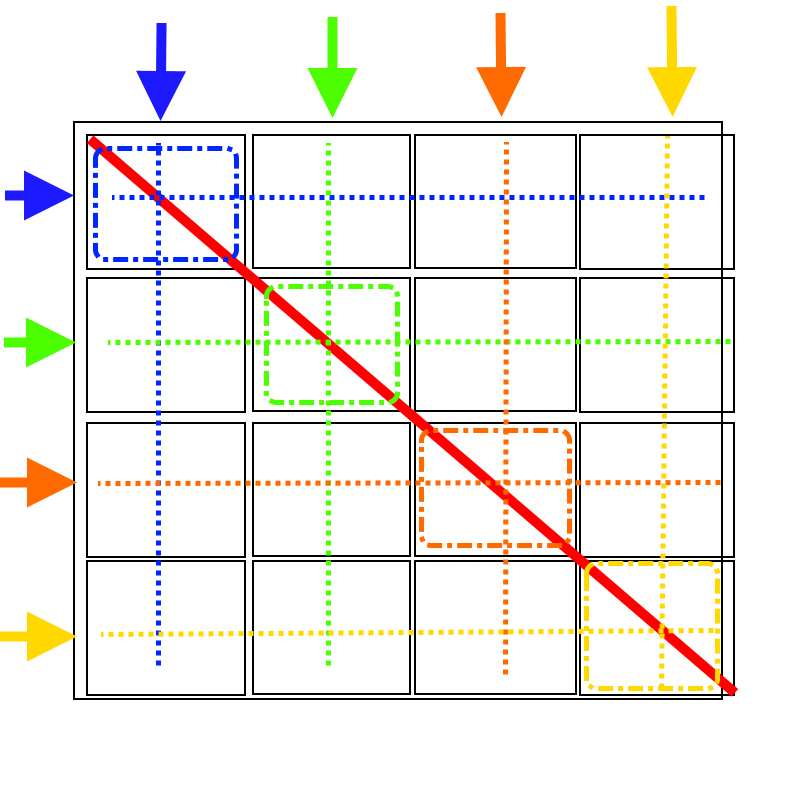
\includegraphics[width=0.6\textwidth]{figs/weighted-matrix}
\label{fig:weighted-matrix}
\caption{Weighting matrix biasing}
\end{figure}
\par
So long each horizontal and vertical weighting groups contributing to each thrust vector, $W_{T_i}\in\mathbb{R}^{3\times 12}$, each have a unit norm, the designed control torque and force inputs will be met. Physically the resultant thrusts and torque (thrust differentials) would be balanced amongst similarly directed components. Furthermore, an additional restraint is that only permissible thrust vector mixings are between opposing pairs; $\vec{T}_1\text{\&}\vec{T}_3$ and $\vec{T}_2\text{\&}\vec{T}_4$. Such a constraint simplifies the time spent optimizing weighting coefficients in Sec:\ref{sec:simulation.allocator}.
\par
The physical consequences of giving priority biasing to thrust vector components in the $\hat{X}_b$ \& $\hat{Y}_b$\footnote{Recalling that the allocator block designs $\vec{T}_{1\rightarrow 4}$ in the body frame, $\in\mathcal{F}^b$. Then the rotation inversion block $R^\dagger(\mathbf{x},\vec{T}_i,t)$ from Eq:\ref{eq:allocator-inersion} finds $(\Omega_i,\lambda_i,\alpha_i)$ to transform $\vec{T}(\Omega_i)$ to the body frame; effectively mapping $\mathcal{F}^{M_i}\rightarrow\mathcal{F}^b$.} directions is that the allocation block prioritizes using pitch or roll servos, $\lambda_i$ \& $\alpha_i$ respectively, before changing the propeller's rotational speed $\Omega_i$. Similarly balancing the of off-diagonal thrust vector mixing blends controller effort amongst opposing actuators. 
\par
The explicit weighting coefficients are to be optimized iteratively in simulation, Sec:\ref{sec:simulation.allocator}; aiming to minimize some performance metric. That metric, which evaluates relative performance of a proposed set of weighting coefficients, is penalized\footnote{More on simulations and optimizations next in Chapter:\ref{ch:simulation}-Simulations \& Results.} from actuator slew rate times and a slack variable norm;
\begin{equation}\label{eq:actuator-penalty}
\int \big(a\norm{t^{\nu_d-\nu_c}-1}+b\norm{s}\big).dt
\end{equation}
Where the integral is run until $t\rightarrow\infty$ over the length of a single simulation cycle. As such, the weighting matrix coefficients try to reduce the transient time taken for the actuator block to settle whilst ensuring stability isn't compromised. Optimization iterations for the weight coefficients are completely independent from the controller coefficient loops to be run in Sec:\ref{sec:simulation.tuning}\ldots
%====================================================
\subsection{Priority Norm Inverse Allocator}
\label{subsec:control.allocation.norminverse}
%====================================================
The last allocator based on typical inversion applies a non-zero preferred actuator position from Eq:\ref{eq:allocation-problem}; or that $u_p\not=\vec{0}\in\mathbb{U}$. The preferred actuator position is the matrix value of $u$ which the allocator naturally tends toward. An obvious choice for that value are the conditions required for stable hovering, those which simply keep the quadcopter airborne. There are however some intricacies which must be discussed with respect to what hovering conditions are.
\par
For a generalized body of weight $m$, a net gravitational force opposes upward movement in the inertial frame; $\vec{M}=[0, 0, -G.m]^T\in\mathcal{F}^I$. At the hover state there are no net forces or torques\footnote{Unwanted system dynamics like torques from an eccentric gravitational center or disturbances are compensated for in a plant dependent control law $\mu\vec{\tau}=h(\mathbf{x}_e,t)$.} acting on the system, all dynamics are balanced. As such the hovering conditions are then simply:
\begin{equation}\label{eq:hover}
\begin{bmatrix}
\mu\vec{F}_p\hspace{3pt}\\
\mu\vec{\tau}_p\hspace{3pt}
\end{bmatrix}
=
\begin{bmatrix}
\vec{M}\hspace{3pt}\\
\vec{0}\hspace{3pt}
\end{bmatrix}~~~~\in\mathcal{F}^I
\end{equation}
\par
\begin{figure}[htbp]
\centering
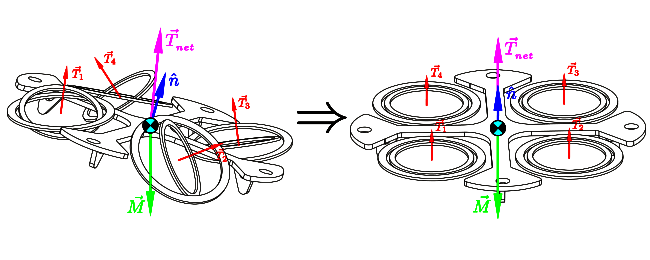
\includegraphics[width=\textwidth]{figs/hover-inertial}
\caption{Hover conditions W.R.T the inertial frame $\mathcal{F}^I$}
\label{fig:hover-inertial}
\end{figure}
\par
However, calculating hover conditions purely in the inertial frame give no indication on what attitude the body has. Two options present themselves on how to solve for hover values. First; take hover conditions with respect to the inertial frame, such that the body's attitude tends to the origin always. The free body diagram in Fig:\ref{fig:hover-inertial} illustrates this. 
\begin{equation}\label{eq:hover-inertial}
\vec{\nu}_I=
\begin{bmatrix}
\mu\vec{F}_p\hspace{3pt}\\
\mu\vec{\tau}_p\hspace{3pt}
\end{bmatrix}
=\begin{bmatrix}
\vec{M}\hspace{3pt}\\
\vec{0}\hspace{3pt}
\end{bmatrix}~~~~\in\mathcal{F}^b
\end{equation}
\par
Conversely, the second option is to take hover conditions with respect to the body frame (Fig:\ref{fig:hover-body}). The difference is that the body's preferred actuator positions are dependent on each instantaneous orientation. That attitude stays constant whilst the actuators are redirected to produce inertial hovering conditions; irrespective of the attitude. The preferred hovering conditions are then always dependent on the commanded attitude trajectory.
\begin{equation}\label{eq:hover-body}
\vec{\nu}_b=
\begin{bmatrix}
\mu\vec{F}_p\hspace{3pt}\\
\mu\vec{\tau}_p\hspace{3pt}
\end{bmatrix}
=\begin{bmatrix}
Q_b^*\otimes\vec{M}\otimes Q_b\\
\vec{0}
\end{bmatrix}~~~~\in\mathcal{F}^b
\end{equation}
\begin{figure}[htbp]
\centering
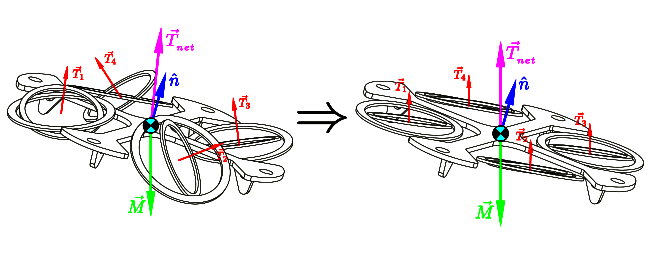
\includegraphics[width=\textwidth]{figs/hover-body}
\caption{Hover conditions W.R.T the body frame $\mathcal{F}^b$}
\label{fig:hover-body}
\end{figure}
\par
Explicit actuator positions are then solved for Eq:\ref{eq:hover-inertial} \& Eq:\ref{eq:hover-body} using pseudo inversion from Eq:\ref{eq:pseudo-inversion}. The two solutions are then as follows:
\begin{subequations}\label{eq:priority-norm}
\begin{equation}\label{eq:priority-norm-inertial}
u_p^I=R^\dagger(\mathbf{x},\big(B^\dagger(\mathbf{x},\vec{\nu}_I,t)\big),t)
\end{equation}
\vspace{-15pt}
\begin{equation}\label{eq:priority-norm-body}
u_p^b=R^\dagger(\mathbf{x},\big(B^\dagger(\mathbf{x},\vec{\nu}_b,t)\big),t)
\end{equation}
\end{subequations}
Where the inverse rotation operator, $R^\dagger$ from Eq:\ref{eq:priority-norm}, is applied to all four thrust vectors produced by the allocation operator $B^\dagger$. Both actuator matrices are then applied to Eq:\ref{eq:inversion} and could be combined with a non-diagonal weighting matrix.
\begin{subequations}
\begin{equation}
\underset{\in\mathbb{U}}{u}=(\mathbb{I}-CB(\mathbf{x},t)\big)u_p+C\vec{\nu}_d
\end{equation}
\vspace{-10pt}
\begin{equation}
C=W^{-1}B^T(\mathbf{x},t)\big(B(\mathbf{x},t)W^{-1}B^T(\mathbf{x},t)\big)^{-1}
\end{equation}
\end{subequations}
The physical consequences of either preferred actuator positions are demonstrated in simulation in Sec:\ref{subsec:simulation.comparison.allocator}. Priority actuator positions aren't simulated together with weighting matrices, the two are compared independently\ldots
%====================================================
\subsection{Non-linear Plant Control Allocation}
\label{subsec:control.allocation.nonlinear}
%====================================================
Despite the added actuation, each complex dynamic response from an actuator excitation is not fully explotited. The dynamics of an actuator's motor module, Sec:\ref{subsec:dynamics.nonlinearities.gyrotorques}, until now has been treated as an element to be compensated for in feedback structure. An alternative approach, seen in Gasco, et al. [2012]\cite{tiltgasco,tiltrihani}, is to use the actuator reactions as additional non-linear actuator plants. In \cite{tiltgasco,tiltrihani} the actuator plants and their resultant dynamics were introduced as additional dimensions to the actuator matrix $u\in\mathbb{U}$. 
\par
Such an approach was achievable because the authors, despite adding two extra degrees of freedom for each propeller, hadn't vectored the propeller thrust. The non-linear proposal here is to first calculate a Pseudo-inversion actuator solution \emph{without} plant compensation\footnote{Disregarding $\vec{\tau}_Q,\vec{\tau}_g$ \& $\vec{Q}$.}, then introducing those induced actuator responses from such an excitation to alleviate the control plant requirement. A subsequent revised virtual control plant input is used iteratively to find a subsequent pseudo-inversion solution; the process is cycled until the control requirements are met.
\par
\begin{figure}[hbtp]
\centering
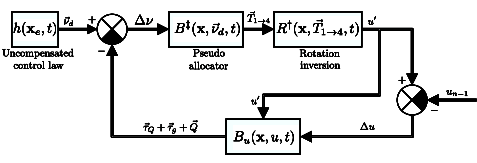
\includegraphics[width=0.6\textwidth]{figs/allocation}
\caption{Allocation loop iteration}
\label{fig:non-linear-allocation}
\end{figure}
In Fig:\ref{fig:non-linear-allocation} the iteration loop is shown, each iteration is run online and settles at a balance point. In the loop, the block $B_u(\mathbf{x},u,t)$ is a combination of non-linear actuator response terms from Eq:\ref{eq:actuator-torque},\ref{eq:grav-torque} \& \ref{eq:aerodynamic-torque}; those being $\vec{\tau}_Q$, $\vec{\tau}_g$ \& $\vec{Q}$ respectively. The settling point, where possible, a portion of the commanded control input $\vec{\nu}_d$ is achieved from the otherwise compensated for actuator response dynamics.

%====================================================
\subsection{Online Optimized Secondary Goal Allocator}
\label{subsec:control.allocation.online}
%====================================================